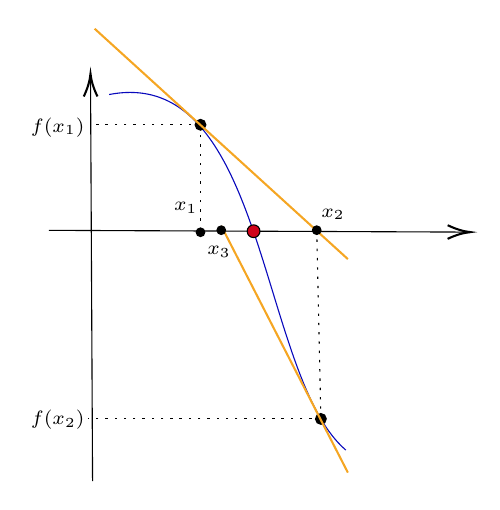
\begin{tikzpicture}[x=0.75pt,y=0.75pt,yscale=-1,xscale=1]
%uncomment if require: \path (0,300); %set diagram left start at 0, and has height of 300

%Straight Lines [id:da6341696579970126] 
\draw    (53,137) -- (254,137.85) ;
\draw [shift={(256,137.86)}, rotate = 180.24] [color={rgb, 255:red, 0; green, 0; blue, 0 }  ][line width=0.75]    (10.93,-3.29) .. controls (6.95,-1.4) and (3.31,-0.3) .. (0,0) .. controls (3.31,0.3) and (6.95,1.4) .. (10.93,3.29)   ;
%Straight Lines [id:da9386272492750976] 
\draw    (74,257.86) -- (73.01,63.57) ;
\draw [shift={(73,61.57)}, rotate = 89.71] [color={rgb, 255:red, 0; green, 0; blue, 0 }  ][line width=0.75]    (10.93,-3.29) .. controls (6.95,-1.4) and (3.31,-0.3) .. (0,0) .. controls (3.31,0.3) and (6.95,1.4) .. (10.93,3.29)   ;
%Curve Lines [id:da7332771912501077] 
\draw [color={rgb, 255:red, 9; green, 9; blue, 188 }  ,draw opacity=1 ]   (82,71.57) .. controls (158,56.86) and (154,206.86) .. (196,242.86) ;
%Straight Lines [id:da6694568846719067] 
\draw  [dash pattern={on 0.84pt off 2.51pt}]  (126,136.86) -- (126,86.14) ;
\draw [shift={(126,86.14)}, rotate = 270] [color={rgb, 255:red, 0; green, 0; blue, 0 }  ][fill={rgb, 255:red, 0; green, 0; blue, 0 }  ][line width=0.75]      (0, 0) circle [x radius= 2.34, y radius= 2.34]   ;
%Straight Lines [id:da32648674551759416] 
\draw  [dash pattern={on 0.84pt off 2.51pt}]  (126,86.14) -- (73,86.14) ;
%Shape: Circle [id:dp5859673038412545] 
\draw  [fill={rgb, 255:red, 208; green, 2; blue, 27 }  ,fill opacity=1 ] (148.5,137.43) .. controls (148.5,135.73) and (149.88,134.36) .. (151.57,134.36) .. controls (153.27,134.36) and (154.64,135.73) .. (154.64,137.43) .. controls (154.64,139.12) and (153.27,140.5) .. (151.57,140.5) .. controls (149.88,140.5) and (148.5,139.12) .. (148.5,137.43) -- cycle ;
%Straight Lines [id:da10660529376202699] 
\draw [color={rgb, 255:red, 245; green, 166; blue, 35 }  ,draw opacity=1 ][line width=0.75]    (75,39.86) -- (197,150.86) ;
%Shape: Circle [id:dp40229126767091916] 
\draw  [fill={rgb, 255:red, 0; green, 0; blue, 0 }  ,fill opacity=1 ] (123.93,137.93) .. controls (123.93,136.78) and (124.86,135.86) .. (126,135.86) .. controls (127.14,135.86) and (128.07,136.78) .. (128.07,137.93) .. controls (128.07,139.07) and (127.14,140) .. (126,140) .. controls (124.86,140) and (123.93,139.07) .. (123.93,137.93) -- cycle ;
%Shape: Circle [id:dp3954498218929916] 
\draw  [fill={rgb, 255:red, 0; green, 0; blue, 0 }  ,fill opacity=1 ] (179.93,136.93) .. controls (179.93,135.78) and (180.86,134.86) .. (182,134.86) .. controls (183.14,134.86) and (184.07,135.78) .. (184.07,136.93) .. controls (184.07,138.07) and (183.14,139) .. (182,139) .. controls (180.86,139) and (179.93,138.07) .. (179.93,136.93) -- cycle ;
%Straight Lines [id:da6934090507517374] 
\draw  [dash pattern={on 0.84pt off 2.51pt}]  (182,136.93) -- (184,227.86) ;
\draw [shift={(184,227.86)}, rotate = 88.74] [color={rgb, 255:red, 0; green, 0; blue, 0 }  ][fill={rgb, 255:red, 0; green, 0; blue, 0 }  ][line width=0.75]      (0, 0) circle [x radius= 2.34, y radius= 2.34]   ;
%Straight Lines [id:da1537553578982449] 
\draw  [dash pattern={on 0.84pt off 2.51pt}]  (184,227.86) -- (72,227.86) ;
%Straight Lines [id:da37580887976486443] 
\draw [color={rgb, 255:red, 245; green, 166; blue, 35 }  ,draw opacity=1 ][line width=0.75]    (136,134.86) -- (197,253.71) ;
%Shape: Circle [id:dp2674385235762444] 
\draw  [fill={rgb, 255:red, 0; green, 0; blue, 0 }  ,fill opacity=1 ] (133.93,136.93) .. controls (133.93,135.78) and (134.86,134.86) .. (136,134.86) .. controls (137.14,134.86) and (138.07,135.78) .. (138.07,136.93) .. controls (138.07,138.07) and (137.14,139) .. (136,139) .. controls (134.86,139) and (133.93,138.07) .. (133.93,136.93) -- cycle ;

% Text Node
\draw (112,122.4) node [anchor=north west][inner sep=0.75pt]  [font=\scriptsize]  {$x_{1}$};
% Text Node
\draw (43,81.4) node [anchor=north west][inner sep=0.75pt]  [font=\scriptsize]  {$f( x_{1})$};
% Text Node
\draw (183,125.4) node [anchor=north west][inner sep=0.75pt]  [font=\scriptsize]  {$x_{2}$};
% Text Node
\draw (43,222.4) node [anchor=north west][inner sep=0.75pt]  [font=\scriptsize]  {$f( x_{2})$};
% Text Node
\draw (128,143.4) node [anchor=north west][inner sep=0.75pt]  [font=\scriptsize]  {$x_{3}$};


\end{tikzpicture}
